\documentclass[8pt]{beamer}
\setbeamerfont{institute}{size=\small}

\newif\ifplacelogo % create a new conditional
\placelogotrue % set it to true

\usetheme{Warsaw}
\usecolortheme{rose}
\usepackage{multicol}
\usepackage{epstopdf}
\usepackage{textcomp}
\usepackage{adjustbox}
\usepackage[italic]{hepnames}
\usepackage{bbding} % for special charachters e.g. for itemize (ftp://ftp.dante.de/tex-archive/fonts/bbding/bbding.pdf)
\usepackage{xcolor}
\usepackage{pdfpages}

% remove navigation buttons
% \beamertemplatenavigationsymbolsempty

% TikZ includes!!!
\usepackage{tikz}
\usepackage[compat=1.1.0]{tikz-feynman}
\usetikzlibrary{backgrounds}
\tikzstyle{every picture}+=[remember picture]
\input{../latexHelpScripts/tikzGrid.tex}

\newcommand{\myCenterBox}[2][pink] {
   {\centering
    \noindent\colorbox{#1}{
	\textbf{#2}
    }\par
  }
}

\newcommand{\mySmallCenterBox}[2][pink] {
   {\centering
    \noindent\colorbox{#1}{
	\textbf{{\small #2}}
    }\par
  }
}

\newcommand{\myVerySmallCenterBox}[2][pink] {
   {\centering
    \noindent\colorbox{#1}{
	\textbf{{\scriptsize #2}}
    }\par
  }
}

\newcommand{\myBox}[2][pink] {
    \noindent\colorbox{#1}{
	\textbf{#2}
    }\par
}

\newcommand{\mySmallBox}[2][pink] {
    \noindent\colorbox{#1}{
	\textbf{{\small #2}}
    }\par
}

\newcommand{\myVerySmallBox}[2][pink] {
    \noindent\colorbox{#1}{
	\textbf{{\scriptsize #2}}
    }\par
}

% do not use backup slides in page counter
\newcommand{\backupbegin}{
   \newcounter{finalframe}
   \setcounter{finalframe}{\value{framenumber}}
}
\newcommand{\backupend}{
   \setcounter{framenumber}{\value{finalframe}}
}

% custom colors
\definecolor{olive}{rgb}{0.3, 0.4, .1}
\definecolor{fore}{RGB}{249,242,215}
\definecolor{back}{RGB}{51,51,51}
\definecolor{title}{RGB}{255,0,90}
\definecolor{dgreen}{rgb}{0.,0.6,0.}
\definecolor{gold}{rgb}{1.,0.84,0.}
\definecolor{JungleGreen}{cmyk}{0.99,0,0.52,0}
\definecolor{BlueGreen}{cmyk}{0.85,0,0.33,0}
\definecolor{RawSienna}{cmyk}{0,0.72,1,0.45}
\definecolor{Magenta}{cmyk}{0,1,0,0}

\begin{document}
% custom commands for positioning of plots
\newcommand{\yRefPosOne}{0.0}
\newcommand{\xRefPosOne}{0.0}
\newcommand{\yRefPosTwo}{0.0}
\newcommand{\xRefPosTwo}{0.0}
\newcommand{\yRefIncrementOne}{0.0}
\newcommand{\xRefIncrementOne}{0.0}
\newcommand{\yRefIncrementTwo}{0.0}
\newcommand{\xRefIncrementTwo}{0.0}

\DeclareGraphicsExtensions{{.pdf},{.png}}
\graphicspath{{/home/oviazlo/Desktop/beamerPresentations/FCCee/pictures/}}



\title[FCCee tracking \hspace{17em}\insertframenumber/
\inserttotalframenumber]{FCCee tracking}


	\author{Oleksandr Viazlo}
	\institute{FCCee MDI study group meeting}
	\date{05.07.17\\}
% 	\logo{ \ifplacelogo \includegraphics[height=1.8cm]{./pictures/lund_uni-logo_s.pdf} \hspace{0.4cm} \fi}
%   	\frame{\titlepage}

\placelogofalse

\newcommand{\channel}{enuqqbb}
\newcommand{\goodChannel}{$t\bar{t} \longrightarrow W^{+}bW^{-}\bar{b} \longrightarrow q\bar{q}be^{-}\bar{\nu_{e}}\bar{b} + e^{+}\nu_{e}bq\bar{q}\bar{b}$}
\newcommand{\myNodeOne}{\tikz[baseline,inner sep=1pt] \node[anchor=base]}
\newcommand{\myNodeTwo}{\tikz[baseline,inner sep=1pt] \node[anchor=base]}

% For nice block (provided by Oleh)
\tikzstyle{mybox} = [draw=red, fill=blue!1, very thick,
    rectangle, rounded corners, inner sep=5pt, inner ysep=9pt]
\tikzstyle{fancytitle} =[fill=white!15, text=black]


%------------------------------------------------
\begin{frame}
\frametitle{VTX + Tracker coverage} 

\begin{tikzpicture}[overlay]

%% HELPER draw advanced helping grid with axises:
% \draw(0,-4) to[grid with coordinates] (11.5,4);

\renewcommand{\yRefPosOne}{0}
\renewcommand{\xRefPosOne}{5.3}
\renewcommand{\xRefIncrementOne}{5.5}

 \node[inner sep=0pt] (tmp) at (\xRefPosOne-3,\yRefPosOne)
    {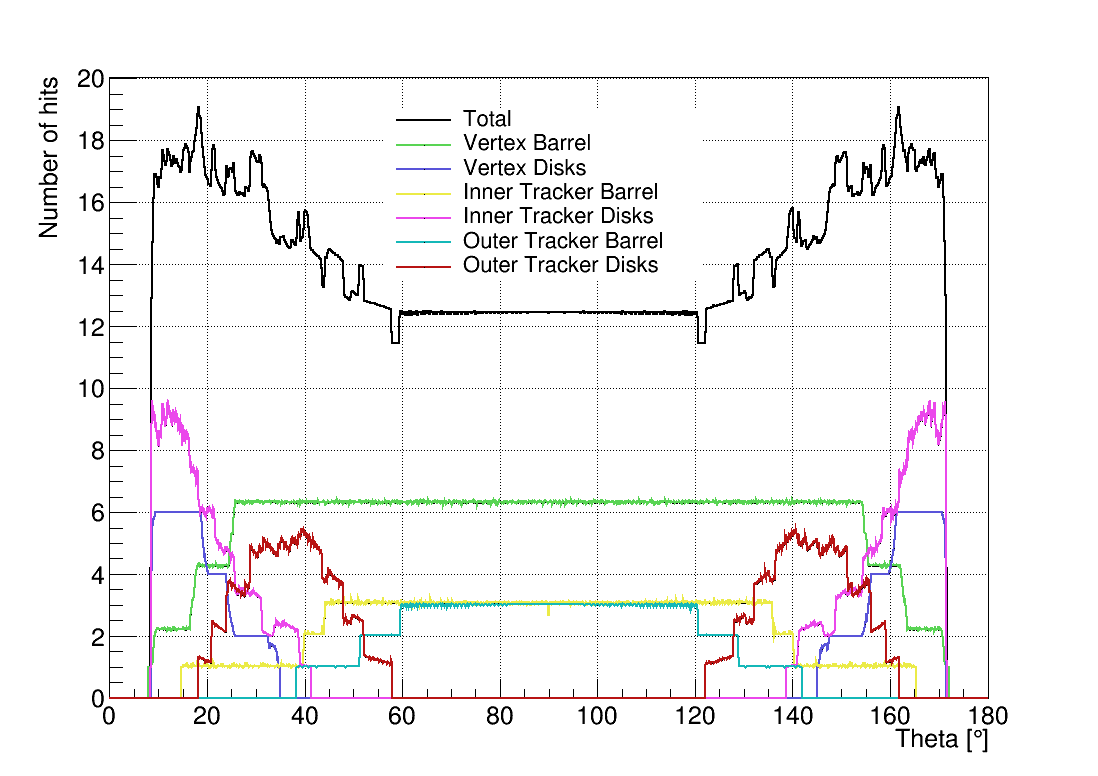
\includegraphics[width=6.8cm]{FCCee_tracking_coverage_v2.png}};
 
 \node[inner sep=0pt] (tmp) at (\xRefPosOne+3.3,\yRefPosOne)
    {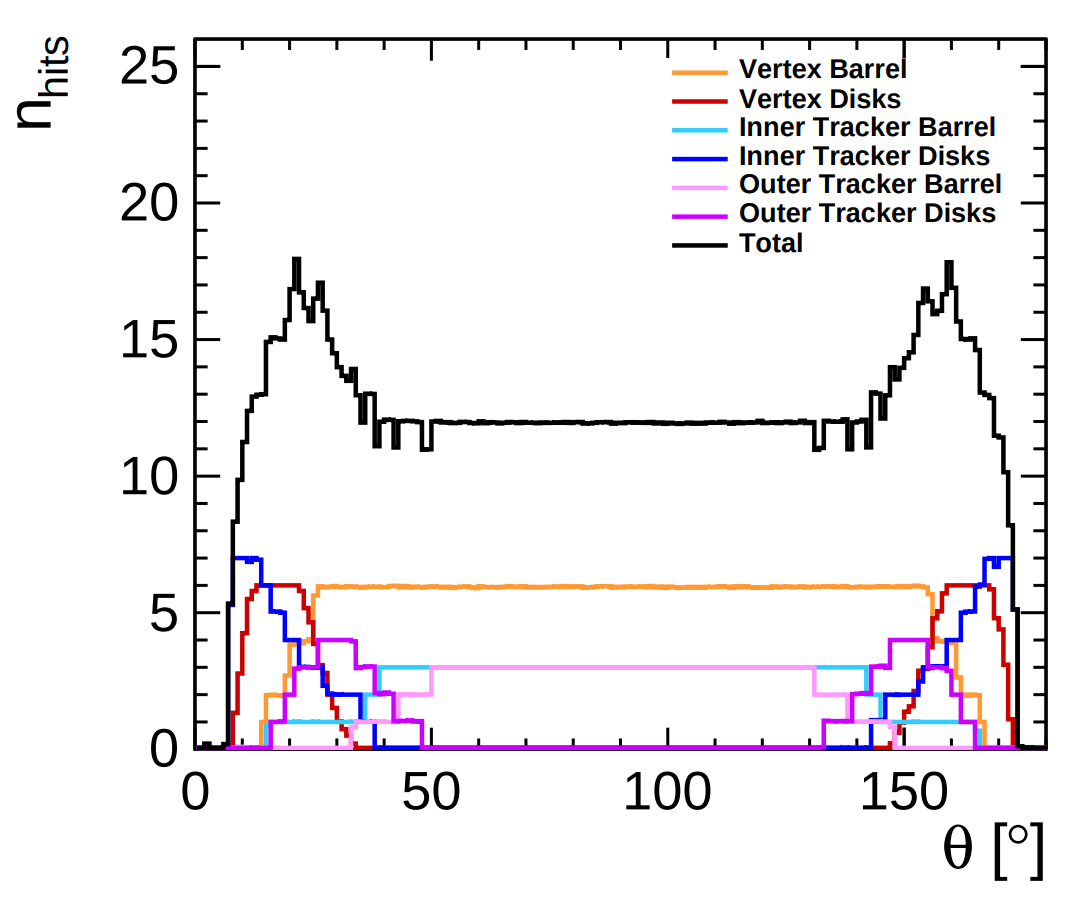
\includegraphics[width=6.8cm]{CLIC_nHits.png}};
    
 \node[inner sep=0pt] (tmp) at (\xRefPosOne-3,\yRefPosOne+3)
    {\mySmallCenterBox{FCCee}};

  \node[inner sep=0pt] (tmp) at (\xRefPosOne+3.3,\yRefPosOne+3)
    {\mySmallCenterBox{CLIC}};
    
%  
%  \node[inner sep=0pt] (tmp) at (\xRefPosOne + \xRefIncrementOne,\yRefPosOne)
%     {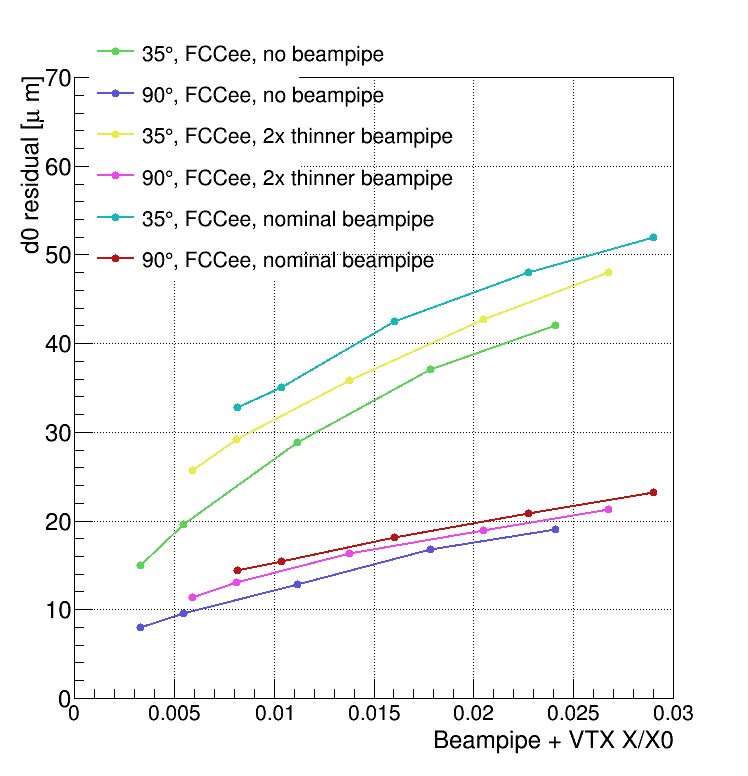
\includegraphics[width=5.0cm]{totalMaterial_WithAndWithoutBeampipe.png}};    

% \node [mybox] at (5.5,\yRefPosOne-4) (box){%
%     \begin{minipage}{10cm}
% %        \scriptsize 
%         \begin{itemize}
%          \item full Tracker
%         \end{itemize}
% 
%     \end{minipage}
% };
% \node[fancytitle, right=15pt] at (box.north west) {Detector};

\end{tikzpicture}
\end{frame}
%------------------------------------------------

%------------------------------------------------
\begin{frame}
\frametitle{FCCee VTX} 

\begin{tikzpicture}[overlay]

%% HELPER draw advanced helping grid with axises:
% \draw(0,-4) to[grid with coordinates] (11.5,4);

\renewcommand{\yRefPosOne}{0}
\renewcommand{\xRefPosOne}{5.6}
\renewcommand{\xRefIncrementOne}{6.0}

 \node[inner sep=0pt] (tmp) at (\xRefPosOne,\yRefPosOne)
    {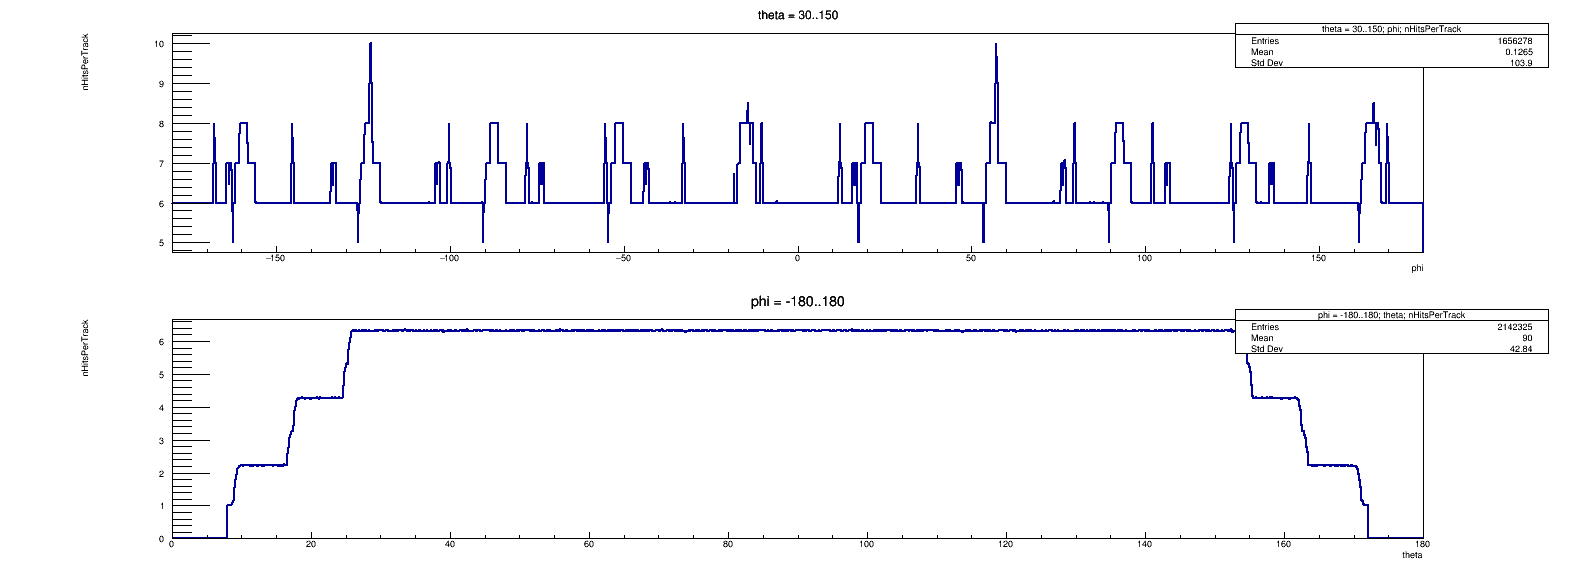
\includegraphics[width=14cm]{VXD_barrel_2.png}};

\node[inner sep=0pt] (tmp) at (\xRefPosOne,\yRefPosOne+2.5)
    {\mySmallCenterBox{Theta: 30..150}};
    
%  \node[inner sep=0pt] (tmp) at (\xRefPosOne + \xRefIncrementOne,\yRefPosOne)
%     {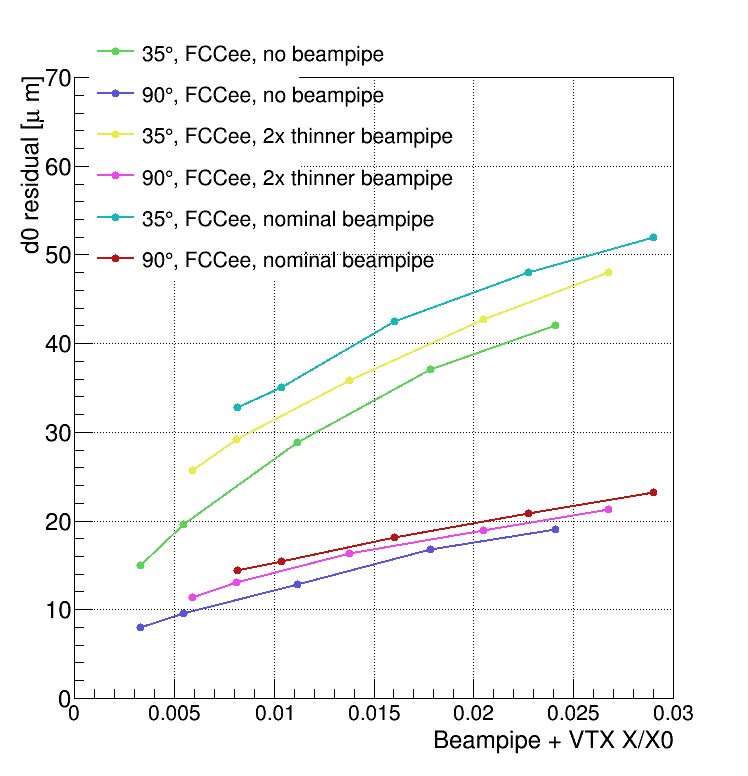
\includegraphics[width=5.0cm]{totalMaterial_WithAndWithoutBeampipe.png}};    

\node [mybox] at (5.5,\yRefPosOne-4) (box){%
    \begin{minipage}{10cm}
%        \scriptsize 
        \begin{itemize}
         \item FCCee VXD Barrel
        \end{itemize}

    \end{minipage}
};
\node[fancytitle, right=15pt] at (box.north west) {Detector};

\end{tikzpicture}
\end{frame}
%------------------------------------------------


%------------------------------------------------
\begin{frame}
\frametitle{FCCee VTX} 

\begin{tikzpicture}[overlay]

%% HELPER draw advanced helping grid with axises:
% \draw(0,-4) to[grid with coordinates] (11.5,4);

\renewcommand{\yRefPosOne}{0}
\renewcommand{\xRefPosOne}{5.6}
\renewcommand{\xRefIncrementOne}{6.0}

 \node[inner sep=0pt] (tmp) at (\xRefPosOne,\yRefPosOne)
    {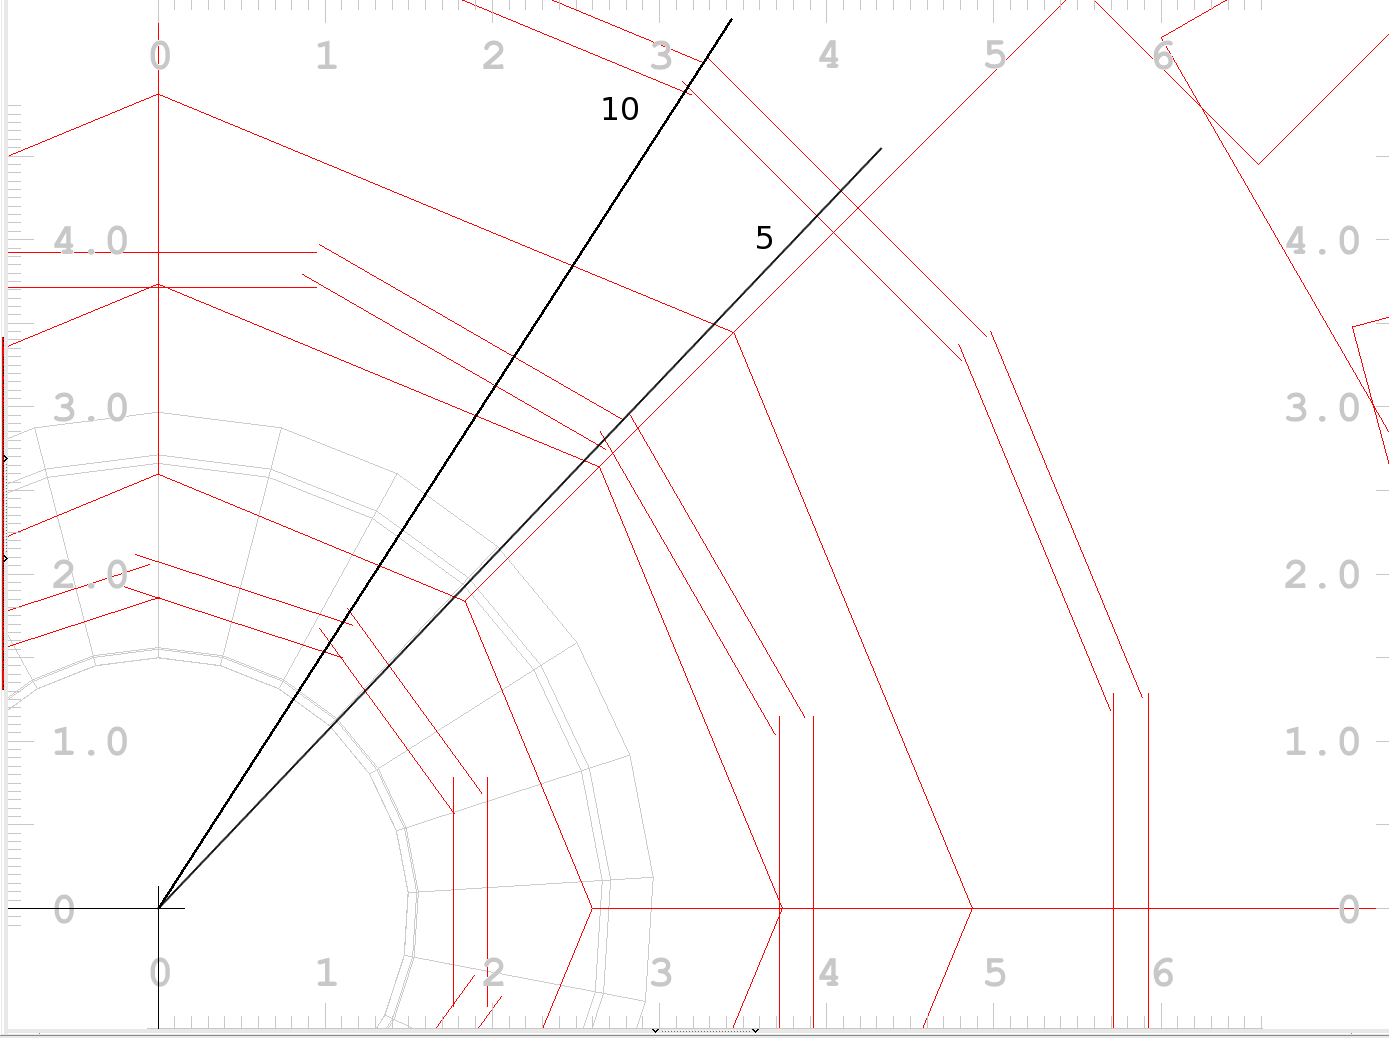
\includegraphics[width=9cm]{VTX_barrel_july10_v2.png}};

    
%  \node[inner sep=0pt] (tmp) at (\xRefPosOne + \xRefIncrementOne,\yRefPosOne)
%     {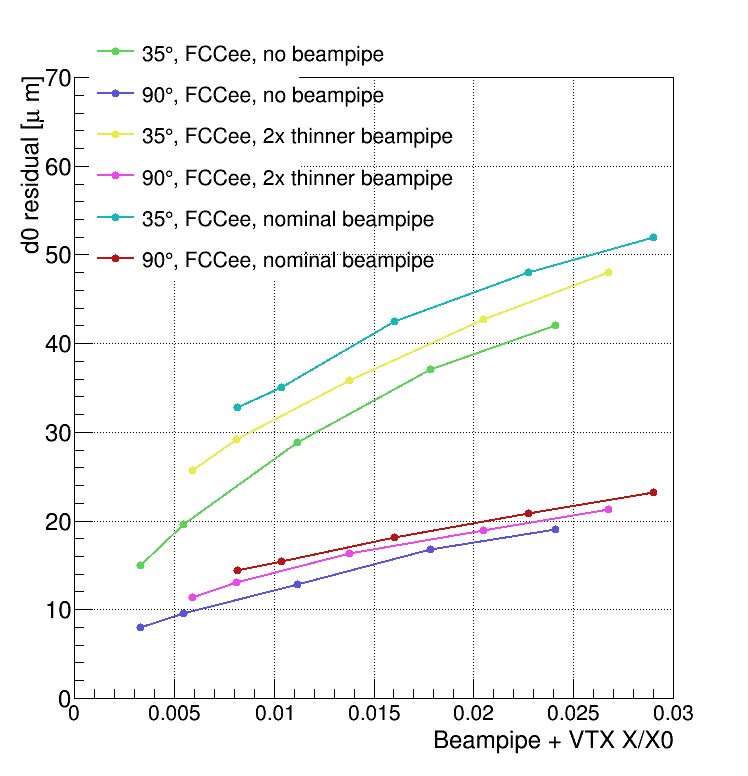
\includegraphics[width=5.0cm]{totalMaterial_WithAndWithoutBeampipe.png}};    

% \node [mybox] at (5.5,\yRefPosOne-4) (box){%
%     \begin{minipage}{10cm}
% %        \scriptsize 
%         \begin{itemize}
%          \item FCCee VXD Barrel
%         \end{itemize}

%     \end{minipage}
% };
% \node[fancytitle, right=15pt] at (box.north west) {Detector};

\end{tikzpicture}
\end{frame}
%------------------------------------------------



%------------------------------------------------
\begin{frame}
\frametitle{FCCee VTX} 

\begin{tikzpicture}[overlay]

%% HELPER draw advanced helping grid with axises:
% \draw(0,-4) to[grid with coordinates] (11.5,4);

\renewcommand{\yRefPosOne}{0}
\renewcommand{\xRefPosOne}{5.3}
\renewcommand{\xRefIncrementOne}{5.5}

 \node[inner sep=0pt] (tmp) at (\xRefPosOne-3,\yRefPosOne)
    {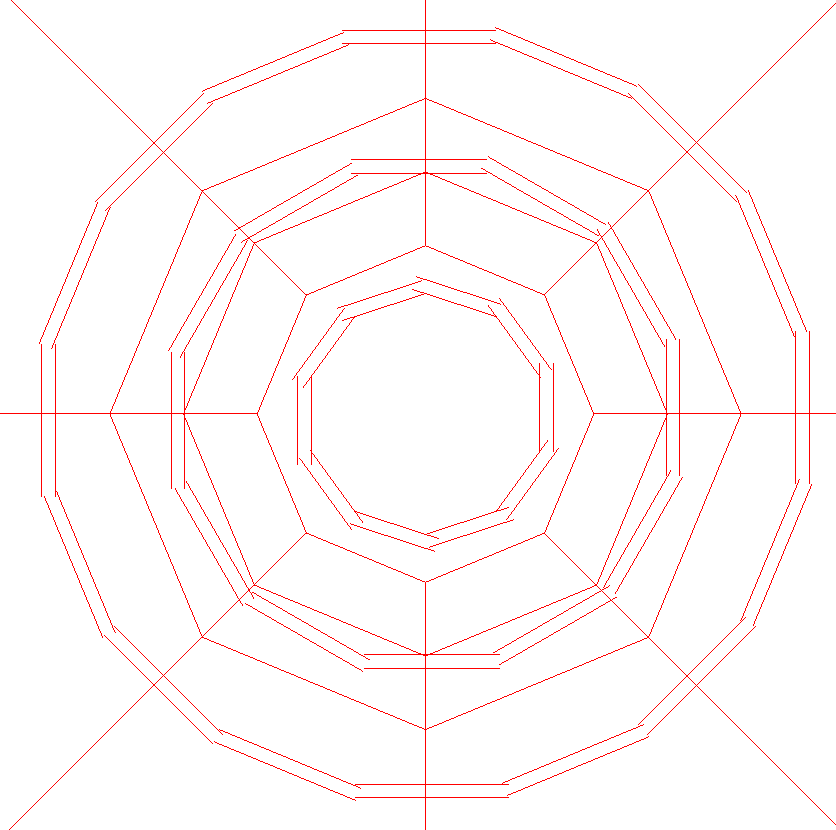
\includegraphics[width=5cm]{layout_FCCee.png}};
 
 \node[inner sep=0pt] (tmp) at (\xRefPosOne+3.3,\yRefPosOne)
    {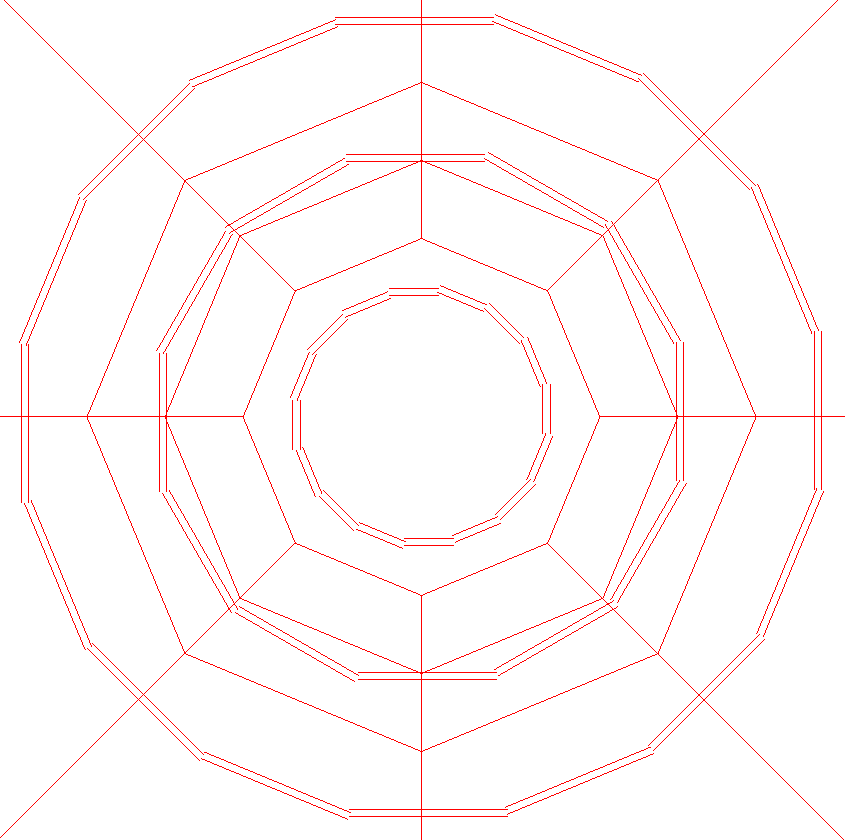
\includegraphics[width=5cm]{layout_clic_scaled.png}};
    
 \node[inner sep=0pt] (tmp) at (\xRefPosOne-3,\yRefPosOne+3)
    {\mySmallCenterBox{FCCee}};

  \node[inner sep=0pt] (tmp) at (\xRefPosOne+3.3,\yRefPosOne+3)
    {\mySmallCenterBox{CLIC scaled}};
   
 \node[inner sep=0pt] (tmp) at (\xRefPosOne,\yRefPosOne-3)
    {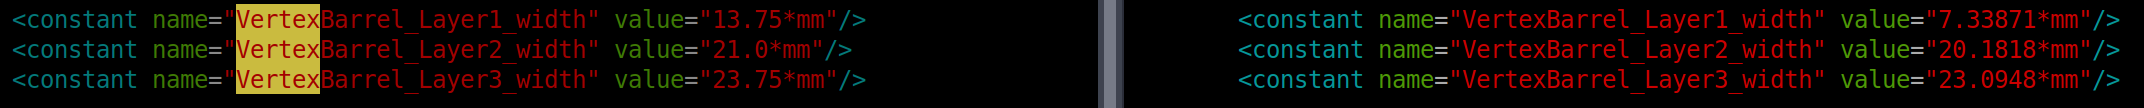
\includegraphics[width=12cm]{vtx_numbers.png}};

   
%  
%  \node[inner sep=0pt] (tmp) at (\xRefPosOne + \xRefIncrementOne,\yRefPosOne)
%     {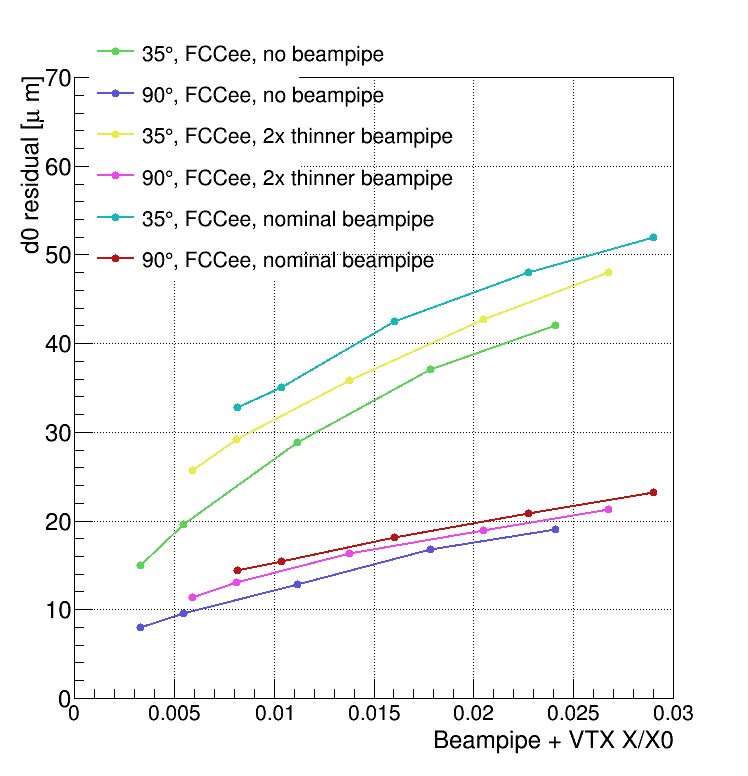
\includegraphics[width=5.0cm]{totalMaterial_WithAndWithoutBeampipe.png}};    

% \node [mybox] at (5.5,\yRefPosOne-4) (box){%
%     \begin{minipage}{10cm}
% %        \scriptsize 
%         \begin{itemize}
%          \item full Tracker
%         \end{itemize}
% 
%     \end{minipage}
% };
% \node[fancytitle, right=15pt] at (box.north west) {Detector};

\end{tikzpicture}
\end{frame}
%------------------------------------------------



\end{document}

